\chapter{Implementation}\label{chapter:implementation}
This chapter goes into the details of our implementation. 
Django follows the MVC pattern in a quite strict
manner, and as a consequence so does our project. In addition to MVC
our project is divided into several Django apps, which are separate
modules containing their own models, views and controllers. 
Each app serve a specific purpose and provide a certain level of
modularity. 

\begin{figure}
	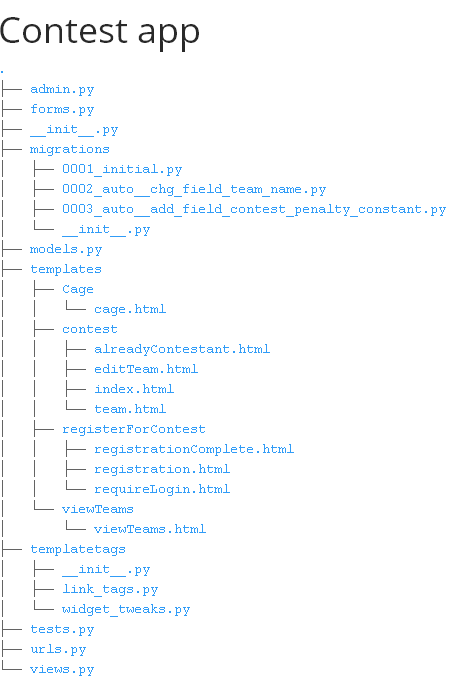
\includegraphics[width=0.8\textwidth]{a07Implementation-img1.png}
	\caption{App overview}
	\label{fig:appOverview}
\end{figure}

\section{Structure}
Figure~\ref{fig:appOverview} shows the directory structure to one of our apps,
all apps follow this structure. An app's root folder contains four files worth
taking a closer look at:

\begin{itemize}
    \item models.py contains the app's models i.e.\ our database entities. Due
        to our site being MVC, every aspect of the site is in some way
        represented by a model defined in a models.py file.

    \item The file views.py defines the app's functions for
    handling requests, called views. Though the naming might be confusing,
    the views defined in this file are not views in the MVC sense of the
    word. The views are in essence MVC controllers. When an HTTP request is
    received by Django it is routed to a specific view, and the view then
    handles the request. Though most views simply serve web pages in
    response to GET requests, there are no limits as to what a view can be
    used for. 

    \item The forms.py file contains a set of Django forms, which are simply
    collections of input fields. The forms can be rendered as HTML, and
    serve as validators of the input received by POSTs. 

    \item This leaves the admin.py file. Django provides a quite modular and
    modifiable admin app for managing other apps. The admin
    page's main functionality is that of viewing, editing,
    creating and deleting models. However, the admin app does not have
    access to all of the models in the system by default. The admin.py file
    is where an app registers which of its models are to be modifiable by
    the admin page, how the models are to be rendered etc.

    \item The apps also contain a templates directory. The templates are in
    essence HTML files extended by Django's template language, making them
    easily processed/modified by Django. These templates corresponds to the MVC
    Views. When a Django view sends a response it is usually by inserting
    dynamic content into a template and then serving the final HTML file as an
    HTTP response. Though not visible in the figure, most of our templates are
    extensions of a global base template, this way redundancy is reduced and
    our user interface stays consistent.
\end{itemize}

\section{contest}
The contest app contains the most fundamental functionality and models for the system,
namely the ones related to creating, hosting, and deleting contests. 
The contest app defines a couple of models
for storing information directly related to a contest, such as sponsor
information, support contact information etc. Just about every
other model in the project is related to the contest models in some way.
A complete overview of the models defined in the contest app can be
found in Appenix~\ref{appendix:ER}.

\section{article}
The article app provides basic functionality for posting news articles.
It contains several different views for looking at articles, lists of
articles etc. For editing articles the app uses a WYSIWYG editor,
available in the admin interface. 

\section{userregistration}
As the name suggests this app handles user creation, deletion and
modification. The majority of this app is an open source app that we
incorporated into our project, however, we made some
modifications of our own. 

\section{teamsubmission}
When a team has reached something they think might be a valid solution
to a problem they submit their source code to the system. The uploaded
source becomes part of a submission model which is part of the
teamsubmission app. This app also defines some models related to the submissions model.

\section{execution}
The system needs a way of handling the submitted source code. For
instance it needs some way of determining which compiler is to be used.
When the source has been built the system needs to know what command is
to be issued to the system to execute the binary. Both of these things
are handled by the execution app. In addition there are restrictions
set to limit the resources available to the submissions, for example
the number of subprocesses, memory allocated etc.


The models defined in teamsubmission and execution can be found in the
Appendix~\ref{appendix:ER}.


\section{node\_manage}
With a well configured system and the previously mentioned apps working
properly, a submitted source file will be stored and the outline of how
the file should be treated will be set when the file is uploaded. The
code for actually performing the actions of building and running is
handled by the node\_manage app. The node\_manage app fetches the
appropriate settings for a submission, and submits it to a FIFO queue.
Our backend consists of several execution nodes connected in a cluster
powered by a framework called Celery. The nodes can be configured to
handle any number of concurrent submissions, and when a node has got
available capacity it fetches another submission from the queue. Celery
relies on the AMQP message passing standard, by means of an open source
message broker system called RabbitMQ.\ All messages passed go through a
broker setup on the same host as the web server, the broker then
distributes the messages to the appropriate host. 

\section{balloon}
When a team has solved a problem, they are to be awarded a helium
balloon. This app enables staff users to view problems that have newly
been solved by a team, send somebody to deliver a balloon, and then
remove them from the list of newly solved. This app simply provides
a custom view in the Django admin page.

\section{changeemail}
Since we had to modify the userregistration app that we incorporated,
not everything worked as we wanted out of the box. An example was
the functionality for changing the email of a contestant, which broke 
the contestant's pending invites. This app provides a fix for that
problem and makes sure that changing email works properly.

\section{judge\_supervise}
This app provides judges with an interface in which they can see all
submitted solutions and statistics for each team. For each submission,
the judges can see compiler errors, execution output and source code. 

\section{clarification}
During a contest questions can be asked by contestants to the staff. If
a problem is ambiguously formulated, or they are experiencing system
errors, these problems can be addressed by requesting a clarification.
The questions are posted publicly on the website, as well as their replies.
